\section{Homework 10}

\subsection{Laplace变换}

(1) $\mathscr{L}(e^{-3t}+1)=\dfrac{1}{s+3}+\dfrac{1}{s}=\dfrac{2s+3}{s(s+3)}(\operatorname{Re}(s)>0$), 
零点为$-3/2$, 极点为$0,-3$.

(2) $\mathscr{L}(4\cos(2t)+2\sin(t))=\dfrac{4}{s^2+4}+\dfrac{2}{s^2+1},(\operatorname{Re}(s)>0)$. 有极点$\pm j, \pm 2j$,
零点$\pm\sqrt{2}j$.

(3) $\mathscr{L}(te^{-2t})=\dfrac{1}{(s+2)^2}$, 极点为$-2$.

(4) $\mathscr{L}(2t^2+3t)=\dfrac{4}{s^3}+\dfrac{3}{s^2}=\dfrac{4+3s}{s^3}$, 极点为$0$, 零点为$-3/4$.

(5) $\mathscr{L}(2\delta(2t-1))=2\cdot (1/2)\cdot e^{-s/2}=e^{-s/2}$, 无零极点.

(6) $\mathscr{L}(\sinh(2t)\cos(t))=\dfrac{1}{2}\mathscr{L}[e^{2t}\cos t - e^{-2t}\cos t]=
\dfrac{2(s^2-5)}{((s-2)^2+1)((s+2)^2+1)}$. 故零点为$\pm\sqrt{5}$, 极点为$2-j,2+j,-2-j,-2+j$.

(7) $\mathscr{L}(\sin^2(\Omega t))=\dfrac12\mathscr{L}[1-\cos(2\Omega t)]=\dfrac{2\Omega^2}{s(s^2+4\Omega^2)}$,
有极点$0$, $\pm 2\Omega j$.

(8) $\mathscr{L}(e^{-3t}\sin 2t)=\dfrac{2}{4+(s+3)^2}$, 极点为$-3\pm2j$.

(9) $\mathscr{L}(\dfrac{e^{-at}+e^{-bt}}{b-a})=\dfrac{1}{b-a}\dfrac{2s+a+b}{(s+a)(s+b)}$, 极点为$-a,-b$, 零点为$
\dfrac{a+b}{2}$.

(10) $\mathscr{L}(e^{-(t+2)}\cos(\Omega t))=e^{-2}\dfrac{s+1}{(s+1)^2+\Omega^2}$. 有零点$-1$, 极点$-1\pm \Omega j$.

(11) $\mathscr{L}((1+4t)e^{-2t})=\dfrac{1}{s+2}+\dfrac{4}{(s+2)^2}=\dfrac{s+6}{(s+2)^2}$, 有零点$-6$, 极点$-2$.

(12) $\mathscr{L}((1-\sin(at))\cdot e^{-bt})=\dfrac{1}{s+b}-\dfrac{a}{(s+b)^2+a^2}$, 有极点$-b,-b\pm aj$, 零点
$-b+\dfrac a 2 \pm \dfrac{\sqrt{3}}{2}aj$.

\subsection{z变换}

(1) $X(z)=\displaystyle\sum_{n=0}^{+\infty}3^{-n}z^{-n}=\dfrac{z}{z-\frac{1}{3}}, |z|>\dfrac{1}{3}$.

(2) $X(z)=\displaystyle\sum_{n=0}^{+\infty}(-2)^{-n}z^{-n}=\dfrac{2z}{2z+1},|z|>\dfrac{1}{2}$.

(3) $X(z)=\displaystyle\sum_{n=-\infty}^{0}(-7)^{-n}z^{-n}=\frac{1}{1+7z},|z|<\frac{1}{7}$.

(4) $X(z)=\displaystyle-2\sum_{n=-\infty}^{-1}2^{-n}z^{-n}=\frac{4z}{2z-1},|z|<\frac{1}{2}$.

(5) $X(z)=\displaystyle\sum_{n=0}^{2}5^{-n}z^{-n}=\frac{25z^2+5z+1}{25z^2},|z|>0$.

(6) $X(z)=\displaystyle\sum_{n=0}^{+\infty}(3^{-n}+2^{-n})z^{-n}=\frac{z}{z-\frac{1}{2}}+\frac{z}
{z-\frac{1}{3}},|z|>\frac{1}{2}$.

(7) $X(z)=1-\frac{1}{2}z^{-4},|z|>0$.

\subsection{Laplace反变换}

(1) $\mathscr{L}^{-1}(\dfrac{1}{s+2})=e^{-2t}$.


(2) $\mathscr{L}^{-1}(\dfrac{2}{s(3s+1)})=\mathscr{L}^{-1}(\dfrac{2}{s}-\dfrac{6}{3s+1})=2-2e^{-t/3}$.


(3) $\mathscr{L}^{-1}(\dfrac{2}{(s+1)(s+3)})=\mathscr{L}^{-1}(\dfrac{1}{s+1}-\dfrac{1}{s+3})=e^{-t}-e^{-3t}$.


(4) $\mathscr{L}^{-1}(2+\dfrac{1}{s^2+16})=\dfrac{1}{4}\sin(4t)+2\delta(t)$.


(5) $\mathscr{L}^{-1}(\dfrac{2}{s(RCs+1)})=2\mathscr{L}^{-1}(\dfrac{1}{s}-\dfrac{1}{s+1/RC})=2-2e^{-t/RC}$.

(6) $\mathscr{L}^{-1}(\dfrac{1}{RCs+1}\cdot\dfrac{s}{s^2+\Omega^2})=\dfrac{1}{RC}e^{-t/(RC)}*\cos(\Omega t)
=\displaystyle\frac{1}{RC}\int_{-\infty}^{+\infty}\cos(\Omega \tau)e^{-(t-\tau)/(RC)}\,\mathrm{d}\tau
$

(7) $\mathscr{L}^{-1}(\dfrac{2s+5}{s^2+3s+2})=\mathscr{L}^{-1}(\dfrac{3}{s+1}-\dfrac{1}{s+2}=e^{-t}-e^{-2t})$.

(8) $\mathscr{L}^{-1}(\dfrac{s+3}{(s+1)^3+2})=\mathscr{L}^{-1}[-\dfrac{1}{s+2}+\dfrac{1}{s+1}-
\dfrac{1}{(s+1)^2}+\dfrac{2}{(s+1)^3}]=-e^{-2t}+e^{-t}-te^{-t}+t^2e^{-t}$.

\subsection{Z反变换}

(1) $x[n]=2\delta[n]$.

(2) $x[n]=\delta[n-5]$.

(3) $x[n]=-3\delta[n-5]+3\delta[n-2]+3\delta[n+1]+\delta[n]$.

(4) $x[n]=Z^{-1}(\dfrac{z}{z-2})=2^nu[n]$.

(5) $x[n]=-3^n u[-n]$.

(6) $x[n]=Z^{-1}[\dfrac{4z}{z+1/2}-\dfrac{3z}{z+1/4}]=4\cdot(-\dfrac{1}{2})^nu[-n-1]-3(-\dfrac{1}{4})^nu[n]$.

(7) $x[n]=Z^{-1}(\dfrac{1}{z-1}-\dfrac{1}{z+1})=-u[n]+(-1)^nu[-n]$.

(8) 

1. $x[n]=\displaystyle\frac{1}{2\pi j}\oint_C \dfrac{5z}{(z-2)(z-1)}z^{n-1}\,\mathrm{d}z=-5u[n]-5\cdot2^nu[-n-1]$.

2. $x[n]=Z^{-1}(-\dfrac{5}{z-1}+10\cdot\dfrac{1}{z-2})=-5u[n]-5\cdot 2^n u[-n-1]$.

3. 如图\ref{fig:10-4-3}, 结果为$x[n]=x_L[n]+x_R[n]=-5u[n]-5\cdot 2^n u[-n-1]$.

\begin{figure*}[htbp]
    \centering
    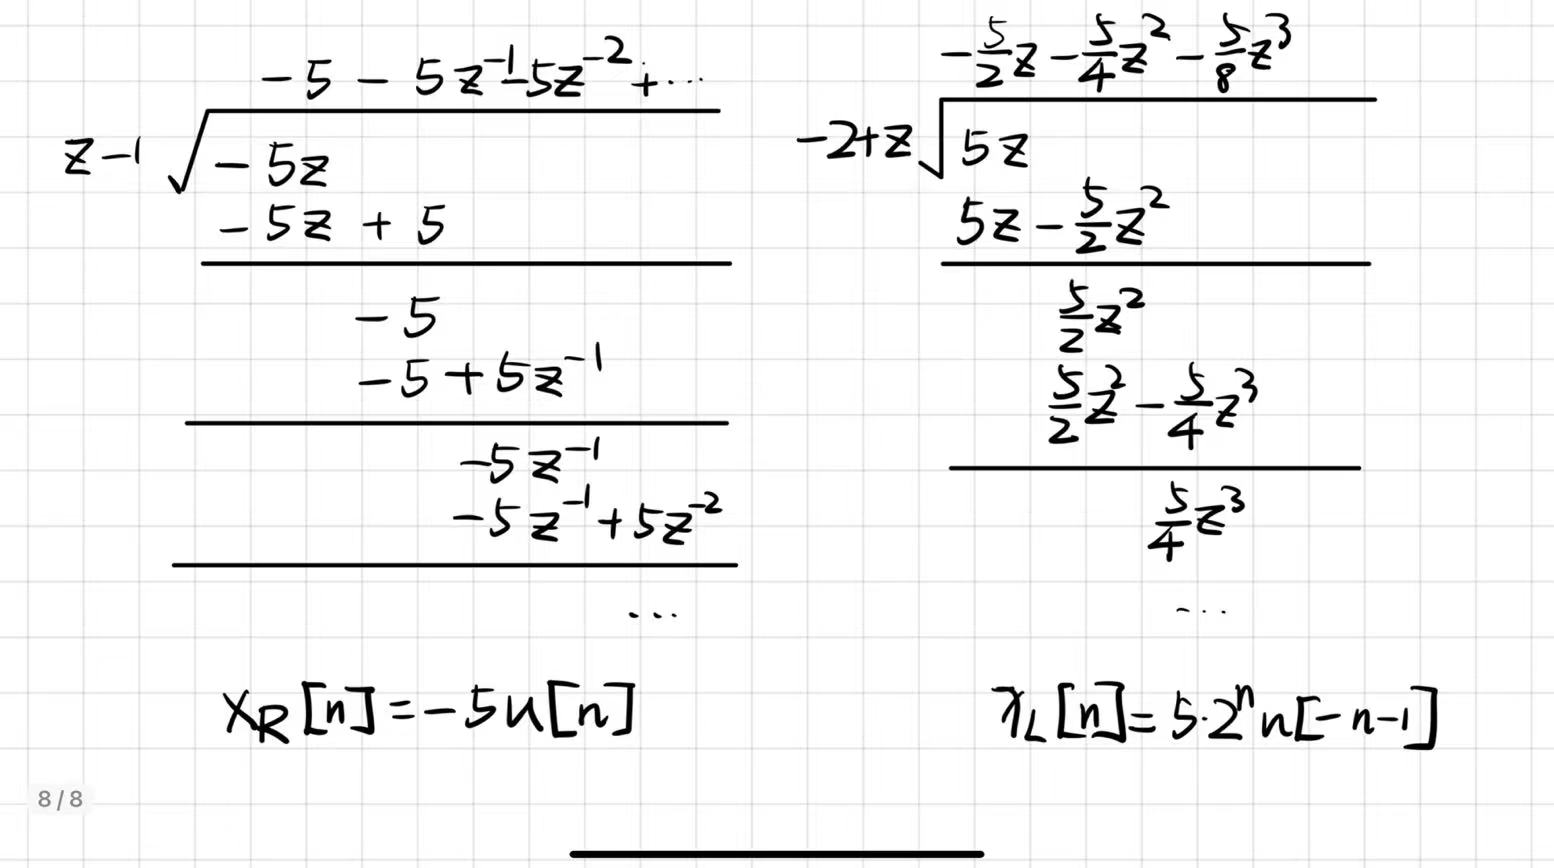
\includegraphics[width=0.7\textwidth]{images/10-4-3.jpg}
    \caption{长除法}\label{fig:10-4-3}
\end{figure*}

\subsection{Laplace变换性质}

\subsubsection{利用Laplace变换性质求解Laplace变换}

(1) $\mathscr{L}[e^{-2t}u(t-2)]=e^{-2(s+2)}\cdot\dfrac{1}{s+2}$.

(2) $\mathscr{L}[f(t)]=\mathscr{L}[\cos(3t)e^{-2t}u(t)]+\mathscr{L}[4\sin te^{-2t}u(t)]=\dfrac{s+2}{(s+2)^2+9}+
\dfrac{4}{(s+2)^2+1}$.

(3) 单个周期的Laplace变换$F(s)=\dfrac{4}{s^2}(1-2e^{-s/4}+2e^{3s/4}-e^{-s})$. 则$L[f(t)]=\displaystyle\sum_{n=0}^{\infty}
F(s)e^{-ns}=\sum_{n=0}^{+\infty}e^{-ns}\dfrac{4}{s^2}(1-2e^{-s/4}+2e^{3s/4}-e^{-s})$.

(4) $\mathscr{L}[2t(1+e^{-3t})u(t)]=\dfrac{1}{s^2}+\dfrac{2}{(s+3)^2}$.

(5) $\mathscr{L}(\dfrac{\sin t}{t}u(t))=\displaystyle\int_{s}^{+\infty}\frac{1}{s^2+1}\,\mathrm{d}s=\frac{\pi}{2}-\arctan(s)$.
